\documentclass[11pt]{article}

\usepackage[a4paper, margin=1in]{geometry}

% FONTS
\usepackage[T1]{fontenc}
%\usepackage{charter}  % Font face
\usepackage[charter]{mathdesign} % charter font with nice maths

% LAYOUT & SPACING
\usepackage{titlesec}
\usepackage{setspace}
\usepackage{fancyhdr}
\usepackage{parskip}  % no paragraph indent + space between paragraphs
%\renewcommand{\baselinestretch}{1.2}  % line spacing
%\spacing{1.2}
\setstretch{1.25}
\setcounter{secnumdepth}{3}  % max. heading depth
\usepackage[colorlinks=true]{hyperref}  % Links in TOC and \refs
\usepackage[titletoc]{appendix}
\usepackage{varwidth}
\usepackage{makecell} % linebreaks in tables
\usepackage[none]{hyphenat} % no hyphenation

% MISC Packages
\usepackage{booktabs}  % table rules
\usepackage{tabularx}
\usepackage{apacite}
\usepackage{xcolor} % Must import BEFORE tcolorbox
\usepackage{tcolorbox}
\usepackage{enumitem}
\usepackage{multirow}
\usepackage{tikz}
\usetikzlibrary{shapes.geometric, arrows, positioning, trees, fit, chains,matrix,calc,arrows.meta,decorations,calligraphy}  % DO NOT use "shadows". It breaks the TOC in half
\usepackage{acronym}
\usepackage{url}
\usepackage{bm} % bold match symbols
\usepackage{longtable}

% HEADER & FOOTER
\pagestyle{fancy}
\fancyhf{}
\rhead{Financial Sentiment Analysis}
\lhead{Moritz Wilksch}
\cfoot{\thepage}

% MISC COMMANDS
%\hypersetup{linktocpage, pdfborder = {0 0 0}} % Links
%\hypersetup{bookmarks=true, bookmarksnumbered=true} % Links in TOC
\hypersetup{
	bookmarks=false,
	bookmarksnumbered=true,
	linktocpage=true,
    colorlinks=false,
    linktoc=all,
    pdfborder={0 0 0},
}
\definecolor{up-blue}{HTML}{00305e}
\renewcommand{\arraystretch}{0.9}  % line spacing WITHIN TABLES
\emergencystretch 5em

% =============================================================================
\begin{document}
% Acronyms, TOC & Style Definitions
\section*{List of Acronyms}
\begin{singlespace}
\begin{acronym}[xxxxxxxxx] % why does this space things?!
	% !!! This needs be sorted manually !!!
	\acro{BERT}{Bidirectional Encoder Representations from Transformers}
	\acro{BoW}{Bag of Words}
	\acro{DL}{Deep Learning}
	\acro{GRU}{Gated Recurrent Unit}
	\acro{LLM}{Large Language Model}
	\acro{LSTM}{Long short-term memory}
	\acro{ML}{Machine Learning}
 	\acro{NLP}{Natural Language Processing}
 	\acro{PCR}{Put/Call Ratio}
 	\acro{RNN}{Recurrent Neural Network}
 	\acro{SA}{Sentiment Analysis}
 	\acro{SM}{Social Media}
 	\acro{SNS}{Social Networking Site}
 	\acro{S\string&P500}{Standard and Poor's 500 index}
 	\acro{SVM}{Support Vector Machine}
 	\acro{US}{United States}
 	\acro{VIX}{Chicago Board Options Exchange Volatility Index}
\end{acronym}
\end{singlespace}
\newpage
\tableofcontents
\newpage
\newtcolorbox{myboxprimary}[2]{title={#1},boxrule=0.5pt,fonttitle=\bfseries,left=2mm,#2}

% grey and white
\newtcolorbox{myboxsecondary}[2]{title={#1},boxrule=0.5pt,colbacktitle=black!10,colback=white,coltitle=black,fonttitle=\bfseries,left=2mm,#2}

\definecolor{lightgrey}{HTML}{EEEEEE}
\definecolor{grey}{HTML}{BBBBBB}
\definecolor{darkgrey}{HTML}{777777}
  % custom tcolorbox styles

% -------------- START CONTENT --------------
\section{Introduction}

The advent of social networking sites (SNS) presents the unique opportunity to tap into an enormous stream of data that users share with the world. However, most of this data comes in the form of images, videos, or text and thus is challenging to analyze. Therefore, researchers utilize automated tools to extract information from these types of media. For images, they can apply object detection to infer what kind of objects are present in a photograph. Speech detection can transcribe spoken words in videos, and named entity recognition can be utilized to recognize entities mentioned in a text. Among these technologies, sentiment analysis has been widely used by scholars and practitioners to derive actionable insights across domains. Also known as ``opinion mining'', sentiment analysis is the practice of automatically extracting sentiments or opinions from short pieces of text. Most of the times, it is measured as a real number on a continuous scale or as a categorical label like ``positive'' or ``negative''. Sentiment obtained from posts on social networks has successfully been used to detect sentiment towards political parties \shortcite{luo2022entity} or consumer products \cite{pontiki2016semeval}. If the per-document sentiment is aggregated over time, it can be used for a plethora of downstream analyses. For example, for the domain of finance, research has shown that sentiment obtained from SNS can help forecast stock market volatility \shortcite{antweiler2004all, audrino2020impact}, trading volume \shortcite{oliveira2017impact}, and even future returns \shortcite{ren2018forecasting, wilksch2022predictive}.\newline
Despite many successful applications, a problem with most sentiment analysis models is that they were designed for working with generic texts. They exploit signaling words like ``good'' or ``bad'' for determining the sentiment of a document. While it has been shown that these models perform excellently on generic social media posts \cite{al2020evaluating}, their performance on domain-specific texts is questionable. Generic sentiment models often misclassify documents containing sentiment that is easy to identify for domain experts. They lack the domain-specific connotation of terms that are only sentiment-laden in a specific domain's context. Because there are few usable domain-specific sentiment models, generic ones are still applied blindly and their output is considered ``ground truth'' for research applications studying large quantities of data. While there are studies researching alternative models for specific domains, few of them publish their models as usable artifacts to enable other researchers to benefit from more accurate sentiment assessments.

This work analyzes and proposes a solution to this issue for the domain of financial market sentiment analysis using a Design Science Research approach. With the goal of building a usable model artifact that can automatically identify an author's opinion about the future of a stock's price, we collect and manually label data to compile a gold-standard dataset of finance-related tweets. We use this data to benchmark existing sentiment models trained on either generic social media data or finance-related texts. After establishing a performance benchmark of models that are popular in the literature, we design and train multiple contending sentiment models. We publish one of the proposed models as an easy-to-use python library such that future studies can utilize it for obtaining more accurate sentiment scores of finance-related social media posts. We hope this improves future research that utilizes the public social media posts of retail investors.

The remainder of this work is structured as follows. The \emph{Theoretical Background} section introduces the concepts needed for automating sentiment analysis using statistical models. It lays out how sentiment is operationalized in the literature, explains the technologies used for automating sentiment analysis, and surveys the literature on existing approaches. Finally, it highlights the research problem we aim to solve by introducing the research questions and the research paradigm we follow to answer them. The \emph{Methodology} section gives a detailed explanation on how the data used for all experiments were collected, labelled, and preprocessed. Furthermore, it lays out the experimental setup we use to train and benchmark all models. Subsequently, we present dataset statistics, an evaluation of model performance and detailed model diagnostics in the \emph{Results} section. We highlight the issue of handling texts with no clear sentiment, provide an example use-case of how the proposed model might be used for future research and introduce the python library that contains the final research artifact. We will discuss the emerging findings in the \emph{Discussion} and provide a final, high-level summary of the work and its findings in the \emph{Conclusion}.
\newpage
\section{Theoretical Background}

\subsection{Financial Posts on Social Media}
\begin{itemize}[noitemsep]
	\item Platforms: Twitter, StockTwits, Reddit, Crypto-specific stuff
	\item Data characteristica: Reddit posts vs. Twitter posts (compare avg. length of each?)
\end{itemize}


\subsection{Sentiment Analysis}  % TODO: wording
\subsubsection{Operationalization of Sentiment}
\begin{itemize}
	\item Definition: ``Opinion'' would be a more accurate term (Munezero, 2014)
	\item Scales: continuous $\in [-1, 1]$, discrete $\in \{pos, neg, neu\}$, 1-5 star reviews \dots
\end{itemize}
\subsubsection{Sentiment in the Financial Context}

Finance-specific, alternative operationalization of sentiment:
\begin{itemize}[noitemsep]
	\item VIX
	\item Fear \& greed index, more in Aggarwal (2018)
	\item Social sentiment @IBKR?
	
\end{itemize}

\subsection{Automated Sentiment Analysis}
\subsubsection{Model Perspective}
\subsubsection{Data Set Perspective}
\subsubsection{Task Perspective}



An example of a prompt to GPT-J \cite{gpt-j}




\subsection{Conceptual Framework}

\newpage
\section{Methodology}
% =======================================================================
\subsection{Data Collection}
% -----------------------------------------------------------------------
\subsubsection{Data Sources}
English-speaking users who discuss finance and investing on online social media platforms in text form do so on three major platforms: Reddit, StockTwits, and Twitter. Reddit is a SNS on which users can create their own communities (``subreddits'') that focus on a specific topic. For example, users have created the subreddits ``Investing'' and ``StockMarket'' to discuss long-term investments and the subreddit ``WallStreetBets'' for posts about high-risk short-term gambles in the market. However, posts on Reddit tend to be much longer than posts on Twitter or StockTwits. Their length would require them to be analyzed on a paragraph- or sentence basis. Since research on SA is mostly focused on document-level analysis, we will not use Reddit posts for this work. The decision between StockTwits and Twitter is harder: posts on both platforms are similar in length and share the usage of cashtags (a ``\$'' sign followed by a ticker symbol) for identifying stocks. We decide to obtain data from Twitter rather than StockTwits for the following reasons:
\begin{enumerate}[noitemsep]
	\item The post volume on Twitter is higher than it is on StockTwits.
	\item The few data sets for SA on financial SM posts that exist use data from StockTwits, hence publishing a data set of Tweets provides more value to the research community.
	\item By using Twitter data for our experiments we can answer RQ4 and compare performances between models and data sources.
\end{enumerate}



% -----------------------------------------------------------------------
\subsubsection{Sampling}
\begin{itemize}[noitemsep]
	\item Twitter: convenience sampling of last $7d$
\end{itemize}


% =======================================================================
\subsection{Data Labelling}

% -----------------------------------------------------------------------
\subsubsection{Task Definition}
\begin{itemize}[noitemsep]
	\item why pos/neg/neu?
	\item codebook!
\end{itemize}



% -----------------------------------------------------------------------
\subsubsection{Data Quality Assessment}  % TODO: wording
\begin{itemize}[noitemsep]
	\item de-dupe
	\item length/cashtag filter
	\item potentially: spam classifier model?
	\item mention: no active learning (\url{https://blog.fastforwardlabs.com/2019/04/02/a-guide-to-learning-with-limited-labeled-data.html})
\end{itemize}




% =======================================================================
\subsection{Data Preprocessing}
\label{section-data-preprocessing}
% -----------------------------------------------------------------------
\subsubsection{Tokenization}
\begin{itemize}[noitemsep]
	\item tokenization
\end{itemize}

% -----------------------------------------------------------------------
\subsubsection{Representation of Text Data}
\begin{itemize}[noitemsep]
	\item vectorizer (TF-IDF?)
	\item Embeddings?
\end{itemize}






% =======================================================================
\subsection{Experiment Design}

%todo: this needs a section for descriptive experiments like bias check and sample tweets demo

% -----------------------------------------------------------------------
\subsubsection{Performance Evaluation}
\begin{itemize}[noitemsep]
	\item cross validation
	\item metrics
\end{itemize}



% -----------------------------------------------------------------------
\subsubsection{Selection of Models}


Models to build:

\begin{table}[!ht]
\centering
	\begin{tabular}{ccc}
		\toprule
%		\textbf{Machine Learning} & \textbf{Deep Learning} & \textbf{Transfer Learning}\\
%		\midrule
%		Naive Bayes & Recurrent NN & BERT \\
%		Logistic Regression & Convolutional NN & DistillBERT \\
%		Random Forest & & roBERTa \\
%		LightGBM & & \\

%		\midrule
		\multicolumn{2}{c}{\textbf{Trained from Scratch}} & \textbf{Transfer Learning}\\
		\cmidrule(r){1-2} \cmidrule(l){3-3}
		\emph{Machine Learning} & \emph{Deep Learning} & \emph{Large Language Models}\\
		\midrule
		Naive Bayes & Recurrent NN & BERT \\
		Logistic Regression & Convolutional NN & DistillBERT \\
		Random Forest? & & roBERTa \\
		LightGBM? & & \\
		\bottomrule		
	\end{tabular}
	\caption{Models to build}
\end{table}



\begin{itemize}[noitemsep]
	\item model types
	\item hyperparameters
\end{itemize}

% -----------------------------------------------------------------------
\subsubsection{Hyperparameters/Search Space?}


\textbf{Finally:} Show a flowchart of everything?







\newpage
\section{Results}

% =======================================================================
\subsection{Dataset Statistics}
Before benchmarking any models on the collected dataset and Fin-SoMe, we assess how similar the datasets are using descriptive statistics. Figure \ref{figure-word-counts} shows the distribution of post lengths measured as the number of words per post. It indicates that tweets tend to be shorter than StockTwits messages on average. However, the distribution of their lengths is right-skewed suggesting that Twitter is occasionally used to share longer posts while StockTwits is not.


\begin{figure}[!ht]
	\includegraphics[width=\textwidth]{assets/images/word_count_distribution.pdf}
	\caption{Number of words per post for tweets (pyFin) and StockTwits posts (Fin-SoMe)}
	\label{figure-word-counts}
\end{figure}

The post length is not the only differentiating characteristic: The distribution of class labels also significantly differs between the two datasets. Within Fin-SoMe, more than 70\% of posts are bullish while only 10\% are bearish. While the data from Twitter also contains more positive than negative tweets, the class ratio is more balanced. However, this does not necessarily imply that posts on StockTwits are generally more positive. The Fin-SoMe dataset either uses slightly different label definitions or contains labeling errors. For example, the post \emph{``\$NXT.X December 28th is the key date. Dec 25-28 this is gonna be wild!''} was labeled as ``bullish''. However, no part of the sentence indicates a clear bullish sentiment. The post author could also expect a stock price drop. Given the ambiguous nature of the text, it would be labeled ``Uncertain'' according to the codebook used in this work.

\begin{figure}[!ht]
	\includegraphics[width=\textwidth]{assets/images/class_distributions.pdf}
	\caption{Distribution of labels within the datasets}
	\label{figure-class-distribution}
\end{figure}

Finally, the vocabulary used in the posts on the two platforms is not identical. The relative frequency of words like ``Elon'', ``chatroom'', ``inflation'', and ``factory'' is between 20 and 50 times higher in the Twitter dataset than it is in the posts from StockTwits. On the other hand, the words ``blackberry'', ``silver'', ``vix'', and ``senate'' are 12 to 25 times more prevalent in StockTwits posts than in tweets. The divergence between the two sets of vocabulary can be explained by platform-specific and temporal differences. Users on Twitter are more prone to interacting with one another, for example by commenting. Additionally, the Fin-SoMe dataset was collected in or before 2020 putting more than two years of time between the posts in both data sets.

% =======================================================================
\subsection{Model Performance Evaluation}

\subsubsection{Optimal Model Configuration}
All subsequently reported results will be based on the optimal model configuration that is found during hyperparameter optimization.
The optimal hyperparameter configuration for each model is presented in Table \ref{table-optimal-hparams}. The chosen hyperparameters suggest that for the ML models subword tokenization outperforms words-based tokenization using character n-grams of size 4. Another notable pattern is the DL models' need for high token dropouts. Both the recurrent neural net and the transformer-based neural net generalize best when 40 - 50\% of the input tokens are dropped. Additionally, the optimal embedding dimensionality is relatively low. A possible cause for this is that complex DL models require stronger regularization to not overfit smaller datasets.

\begin{table}[!ht]
\centering
\small

\begin{tabular}{lccccc}
\toprule
& \multicolumn{5}{c}{\textbf{Model}} \\
 \cmidrule(lr){2-6} 
\textbf{Hyperparameter} & Logistic Regression & SVM & Recurrent NN & Transformer NN & BERT Finetune \\
\midrule

vectorizer\_analyzer & char\_wb & char\_wb & -- & -- & -- \\
vectorizer\_ngram\_range & (4, 4) & (4, 4) & -- & -- & -- \\
vectorizer\_min\_df & 1.02e-06 & 2.87e-05 & -- & -- & -- \\
model\_C & 1.428 & 1.597 & -- & -- & -- \\
model\_kernel & -- & rbf & -- & -- & -- \\
model\_degree & -- & -- & -- & -- & -- \\
\midrule
token\_dropout & -- & -- & 0.498 & 0.439 & -- \\
embedding\_dim & -- & -- & 54 & 72 & -- \\
hidden\_dim & -- & -- & 189 & 237 & 238 \\
dropout & -- & -- & 0.414 & 0.286 & 0.249 \\
gru\_hidden\_dim & -- & -- & 44 & -- & -- \\
dim\_ff & -- & -- & -- & 140 & -- \\

\bottomrule
\end{tabular}
\caption{Optimal hyperparameter configuration for each model}
\label{table-optimal-hparams}
\end{table}




\subsubsection{Performance on the Twitter Dataset}
Figure \ref{figure-model-performance-twitter} displays each model's out-of-sample ROC AUC when applied to the dataset we collected from Twitter. The dictionary-based VADER and NTUSD-Fin perform worst scoring an AUC of 0.578 and 0.590 respectively. The domain-specific NTUSD-Fin outperforms VADER, but only by a small margin. FinBERT and TwitterRoBERTa, on the other hand, perform significantly better by both achieving an AUC score of 0.695.\newline
In comparison, all of the proposed models obtain AUC scores above 0.80. Out of these models, the recurrent neural net performs worst with an AUC of 0.803. It is outperformed by both the fine-tuned BERT model and the transformer-based neural network which score an AUC of 0.814. The two best models are the logistic regression and the SVM model which achieve AUC scores of 0.817 and 0.827 respectively.


\begin{figure}[!ht]
	\includegraphics[width=\textwidth]{assets/images/model_performance_pyfin.pdf}	
	\caption{Out-of-sample model performance on the dataset collected from Twitter}
	\label{figure-model-performance-twitter}
\end{figure}



\subsubsection{Performance on the StockTwits Dataset}
To answer RQ4, we apply all models to the StockTwits posts compiled in the Fin-SoMe dataset. The corresponding model performances are dispalyed in Figure \ref{figure-model-performance-stocktwits}. The existing models' performance hardly changes compared to the ROC AUC on the tweet dataset. VADER now scores a slightly higher AUC of 0.590 while NTUSD-Fin achieves a score of 0.599. TwitterRoBERTa and FinBERT achieve AUC values of 0.705 and 0.710 respectively. On the other hand, all of the proposed models perform significantly worse on Fin-SoMe. The fine-tuned BERT model only scores an AUC of 0.702 while the transformer-based and recurrent neural network reach AUC scores of 0.707 and 0.709 respectively. The two ML models still perform best by obtaining an AUC of 0.727. Despite the relative performance decrease when applied to data from a different source, the proposed ML models still manage to outperform the existing BERT-based models.

\begin{figure}[!ht]
	\includegraphics[width=\textwidth]{assets/images/model_performance_finsome.pdf}	
	\caption{Out-of-sample model performance on Fin-SoMe}
	\label{figure-model-performance-stocktwits}
\end{figure}



\subsubsection{Inference Times}
In times where state-of-the-art language models like GPT-3 require millions of dollars in compute budget for training \cite{gpt3-cost}, it is important to assess the resourcefulness of machine learning models. Therefore, we quantify each models inference speed. Slower models require more compute time which, in a business setting, requires a larger compute budget. Figure \ref{figure-model-inference-times} presents the inference time per sample. Note that the y-axis is log-scaled due to the multiple orders of magnitude that lie between the fastest and the slowest model's speed. All experiments were conducted on a system with an AMD Ryzen 5 3600 CPU and 64GB of RAM.

\begin{figure}[!ht]
	\includegraphics[width=\textwidth]{assets/images/model_inference_time.pdf}	
	\caption{Inference time per sample (ms, log-scaled)}
	\label{figure-model-inference-times}
\end{figure}

VADER and the logistic regression model provide the fastest inference times below 0.1ms per sample. Both of the neural networks that we train from scratch are slower, but still deliver inference times of below 1ms, which is on-par with NTUSD-Fin. The SVM model is roughly 50 times slower than the fastest models at around 2.5ms per sample. Finally, all models that are based on LLMs are multiple orders of magnitude slower than the next quickest contender. At around 100ms per sample, they are more than 1000 times slower than the logistic regression. We have to acknowledge that all neural-network-based models would benefit from being run on a graphics processing unit (GPU). However, \shortciteA{buber2018performance} suggest that GPU utilization can speed up inference by a factor of 4 or 5, which would still leave the LLM-based models far behind all other ones in terms of speed.

\begin{itemize}[noitemsep]
	\item compare model performances on semEval?? financial phrase bank??
	\item mention training times?
\end{itemize}
% =======================================================================
\subsection{Model Diagnostics}
\begin{itemize}[noitemsep]
	\item show demos: engineer categories (e.g. simple stock, options, news headline, ...) 
	\item own models: where do they fail?
	\item SHAP values / most important words
 	\item show the learned word embeddings!
\end{itemize}


% =======================================================================
\subsection{Analyzing Spam Posts(?)}

% -----------------------------------------------------------------------
% =======================================================================
\subsection{pyFin-Sentiment}
reference the python library.


%\begin{figure}[!ht]
	\centering
	\begin{tikzpicture}
		\tikzstyle{mystyle}=[draw,darkgrey,opacity=0,anchor=east]
		\tikzstyle{level1style}=[draw,minimum height=18pt]
		
		\node[mystyle](l1) at (-3.5, 0.5) {Word};
		\node[mystyle](l1) at (-3.5, -1) {Tokens};
		
		\draw
			node[rectangle,draw,line width=1pt,fill=lightgrey](word) at (-0.5,0.5) {university}
			node[level1style](n1) at (-2, -1) {uni}
			node[level1style](n2) at (-1, -1) {niv}		
			node[level1style](n3) at (0, -1) {...}
			node	[level1style](n4) at (1, -1) {ity};
		
		\coordinate[above=0.25cm of n1](c1);
		\coordinate[above=0.25cm of n2](c2);
		\coordinate[above=0.25cm of n3](c3);
		\coordinate[above=0.25cm of n4](c4);
		
		\draw 
			(n1.north) -- (c1) -| (word.south)
			(n2.north) -- (c2) -| (word.south)
			(n3.north) -- (c3) -| (word.south)
			(n4.north) -- (c4) -| (word.south);
		
	\end{tikzpicture}
	\caption{An example tikz figure showing a diagram}
\end{figure}
%
\begin{figure}[!ht]
	\centering
	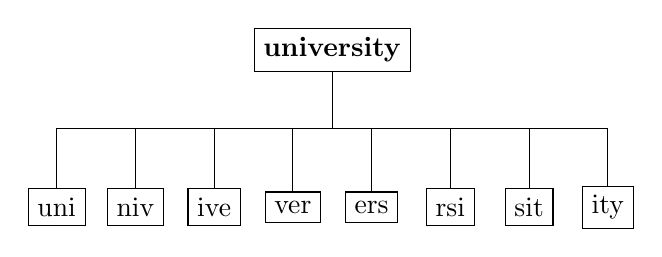
\begin{tikzpicture}
	[
		level 1/.style={level distance=2cm, sibling distance=1cm},
		edge from parent fork down
	]
		\node[draw] {\textbf {university}}
    	child {node[draw] {uni}}
	    child {node[draw] {niv}}
	    child {node[draw] {ive}}
	    child {node[draw] {ver}}
	    child {node[draw] {ers}}
	    child {node[draw] {rsi}}
	    child {node[draw] {sit}}
	    child {node[draw] {ity}};
\end{tikzpicture}
\end{figure}




\newpage

% ---------- Notes for Finalizing --------------
% TODO: check whether each acronym is spelled out at first use!
% TODO: run through grammarly
% TODO: check page numbering starts on introduction page, NOT before

% -------------- START REFERENCES --------------
\bibliography{bibliography/refs}{}
\bibliographystyle{apacite}

% -------------- START APPENDIX --------------
\newpage
\begin{appendices}
\section{Section Heading}
Hello Test
\end{appendices}




\end{document}